\newpage

\section{Actividad 2: Curvas características del SCR}

\subsection{Actividad de Laboratorio}

\begin{itemize}
    \item SCR TIC106D.
    \item Fuente de alimentación DC 0 a 600V.
    \item Dos multímetros.
    \item Potenciómetro de 5k$\Omega$.
    \item Resistores varios.
\end{itemize}

\paragraph{Procedimiento}

Para esta actividad se implementó el circuito mostrado anteriormente.

Primero fijamos un valor de $I_G$ y variamos $V_{CC}$ hasta ovservar el disparo del SCR, anotando los valores de $V_{AK}$ e $I_{AK}$.


\begin{table}[ht]
\centering
\setlength{\tabcolsep}{5pt} 
\renewcommand{\arraystretch}{1.1}

\begin{minipage}[t]{0.5\textwidth} 
\centering
\small

\label{tab:datos_adaptados}
\begin{tabular}{|c|c|c|c|}
\hline
\rowcolor[HTML]{9AFF99}
$\mathbf{I_G\ [\mu A]}$ & $\mathbf{V_{CC}\ [V]}$ & $\mathbf{I_{AK}\ [mA]}$ & $\mathbf{V_{AK}\ [V]}$ \\
\hline
% --- Datos de la tabla original ---
10 & 95 & 19.8 & 1.25 \\ \hline
20 & 80 & 16.5 & 1.10 \\ \hline
30 & 65 & 13.0 & 0.95 \\ \hline
40 & 55 & 10.2 & 0.84 \\ \hline
50 & 45 & 7.6 & 0.75 \\ \hline
\end{tabular}

\caption{Datos de Medición}
\end{minipage}


\end{table}

Ahora realizamos el mismo procedimiento pero para cada vez un valor de $I_G$ variamos $V_{CC}$ para obtener $V_{AK}$ desde 0 hasta 15V.\\
\begin{table}[ht]
\centering
\setlength{\tabcolsep}{4pt} % Ajuste un poco el espacio, ya no es crítico
\renewcommand{\arraystretch}{0.9} 
\footnotesize % Usamos \footnotesize, que es más legible que \scriptsize

\caption{Tabla 3: Datos de Medición (Curvas I-V)}
\label{tab:datos_curvas_dividida}

\subcaption*{Parte 1: $I_G = 50\,\mu A$ a $I_G = 30\,\mu A$} % Subtítulo para la primera parte

\begin{tabular}{|*{6}{c|}} % 6 columnas en total (3 grupos de 2)
\hline
% --- Fila 1: Encabezado Principal (FFCE93) ---
\rowcolor[HTML]{FFCE93}
\multicolumn{2}{|c|}{\cellcolor[HTML]{FFCE93}$I_G = 50\,\mu\text{A}$} & 
\multicolumn{2}{c|}{\cellcolor[HTML]{FFCE93}$I_G = 40\,\mu\text{A}$} & 
\multicolumn{2}{c|}{\cellcolor[HTML]{FFCE93}$I_G = 30\,\mu\text{A}$} \\ 
\hline
% --- Fila 2: Sub-encabezado (9AFF99) ---
\rowcolor[HTML]{9AFF99}
$V_{AK}\ [\text{V}]$ & $I_{AK}$ & 
$V_{AK}\ [\text{V}]$ & $I_{AK}$ & 
$V_{AK}\ [\text{V}]$ & $I_{AK}$ \\ 
\hline
% --- Datos: Parte 1 ---
$300\,\text{mV}$ & $180\,\text{nA}$ & $300\,\text{mV}$ & $180\,\text{nA}$ & $300\,\text{mV}$ & $187\,\text{nA}$ \\ \hline
$600\,\text{mV}$ & $373\,\text{nA}$ & $600\,\text{mV}$ & $373\,\text{nA}$ & $600\,\text{mV}$ & $373\,\text{nA}$ \\ \hline
$800\,\text{mV}$ & $13.48\,\mu\text{A}$ & $700\,\text{mV}$ & $430\,\text{nA}$ & $700\,\text{mV}$ & $436\,\text{nA}$ \\ \hline
$900\,\text{mV}$ & $31.6\,\mu\text{A}$ & $800\,\text{mV}$ & $13\,\mu\text{A}$ & $900\,\text{mV}$ & $14\,\mu\text{A}$ \\ \hline
$1.0\,\text{V}$ & $45.26\,\mu\text{A}$ & $1.0\,\text{V}$ & $45.26\,\mu\text{A}$ & $1.0\,\text{V}$ & $38.53\,\mu\text{A}$ \\ \hline
$1.2\,\text{V}$ & $66.9\,\mu\text{A}$ & $1.1\,\text{V}$ & $53\,\mu\text{A}$ & $1.2\,\text{V}$ & $40.06\,\mu\text{A}$ \\ \hline
$1.5\,\text{V}$ & $87.4\,\mu\text{A}$ & $1.2\,\text{V}$ & $53.9\,\mu\text{A}$ & $1.4\,\text{V}$ & $42.07\,\mu\text{A}$ \\ \hline
\end{tabular}
\vspace{0.5em} % Pequeño espacio entre tablas

\subcaption*{Parte 2: $I_G = 20\,\mu A$ a $I_G = 10\,\mu A$} % Subtítulo para la segunda parte

\begin{tabular}{|*{4}{c|}} % 4 columnas en total (2 grupos de 2)
\hline
% --- Fila 1: Encabezado Principal (FFCE93) ---
\rowcolor[HTML]{FFCE93}
\multicolumn{2}{|c|}{\cellcolor[HTML]{FFCE93}$I_G = 20\,\mu\text{A}$} & 
\multicolumn{2}{c|}{\cellcolor[HTML]{FFCE93}$I_G = 10\,\mu\text{A}$} \\ 
\hline
% --- Fila 2: Sub-encabezado (9AFF99) ---
\rowcolor[HTML]{9AFF99}
$V_{AK}\ [\text{V}]$ & $I_{AK}$ & 
$V_{AK}\ [\text{V}]$ & $I_{AK}$ \\ 
\hline
% --- Datos: Parte 2 ---
$400\,\text{mV}$ & $250\,\text{nA}$ & $200\,\text{mV}$ & $124\,\text{nA}$ \\ \hline
$700\,\text{mV}$ & $436\,\text{nA}$ & $600\,\text{mV}$ & $373\,\text{nA}$ \\ \hline
$800\,\text{mV}$ & $11.3\,\mu\text{A}$ & $700\,\text{mV}$ & $436\,\text{nA}$ \\ \hline
$900\,\text{mV}$ & $23.5\,\mu\text{A}$ & $800\,\text{mV}$ & $8.5\,\mu\text{A}$ \\ \hline
$1.2\,\text{V}$ & $27.33\,\mu\text{A}$ & $1.1\,\text{V}$ & $14\,\mu\text{A}$ \\ \hline
$1.4\,\text{V}$ & $27.5\,\mu\text{A}$ & $1.4\,\text{V}$ & $14.5\,\mu\text{A}$ \\ \hline
$1.5\,\text{V}$ & $27.6\,\mu\text{A}$ & $2.0\,\text{V}$ & $22\,\mu\text{A}$ \\ \hline
\end{tabular}

\end{table}

En base a los datos obtenidos, podemos graficar las curvas $I_{AK}$ vs $V_{AK}$ para los distintos valores de $I_G$.\\

\begin{figure}[ht]
\centering
\pgfplotsset{compat=1.18}
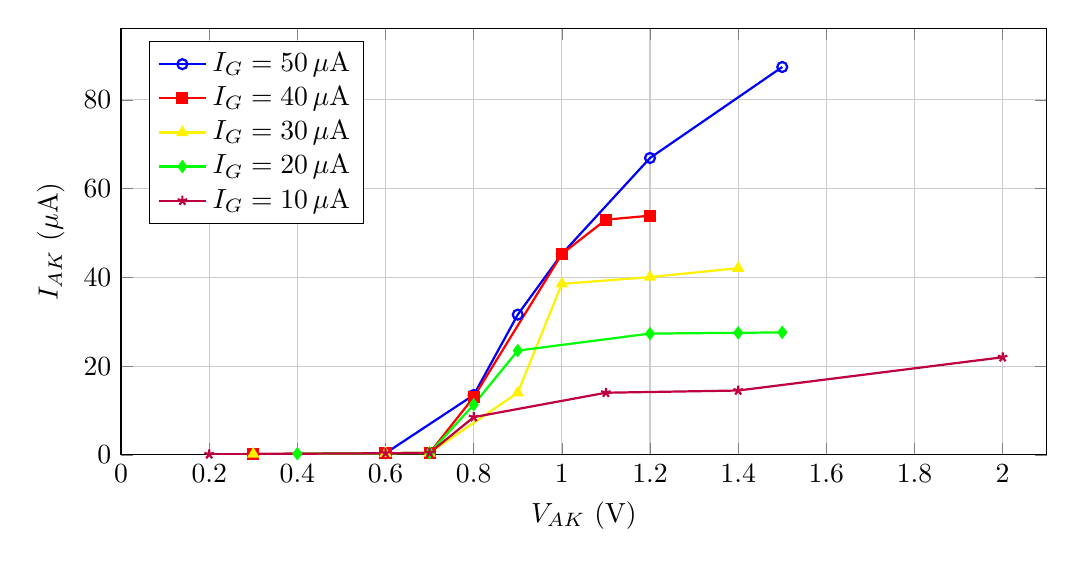
\begin{tikzpicture}
\begin{axis}[
    width=1.1\linewidth,
    height=7cm,
    xlabel={$V_{AK}$ (V)},
    ylabel={$I_{AK}$ ($\mu$A)},
    xmin=0, xmax=2.1,
    ymin=0,
    grid=both,
    major grid style={gray!40},
    minor grid style={gray!10},
    legend cell align=left,
    legend pos=north west,
    cycle list name=color list,
    mark options={scale=0.9}
]

% I_G = 50 μA
\addplot[thick,mark=o,blue] coordinates {
    (0.300,0.18) (0.600,0.373) (0.800,13.48) (0.900,31.6) (1.000,45.26) (1.200,66.9) (1.500,87.4)
};
\addlegendentry{$I_G=50\,\mu$A}

% I_G = 40 μA
\addplot[thick,mark=square*,red] coordinates {
    (0.300,0.18) (0.600,0.373) (0.700,0.43) (0.800,13.0) (1.000,45.26) (1.100,53.0) (1.200,53.9)
};
\addlegendentry{$I_G=40\,\mu$A}

% I_G = 30 μA
\addplot[thick,mark=triangle*,yellow] coordinates {
    (0.300,0.187) (0.600,0.373) (0.700,0.436) (0.900,14.0) (1.000,38.53) (1.200,40.06) (1.400,42.07)
};
\addlegendentry{$I_G=30\,\mu$A}

% I_G = 20 μA
\addplot[thick,mark=diamond*,green] coordinates {
    (0.400,0.25) (0.700,0.436) (0.800,11.3) (0.900,23.5) (1.200,27.33) (1.400,27.5) (1.500,27.6)
};
\addlegendentry{$I_G=20\,\mu$A}

% I_G = 10 μA
\addplot[thick,mark=star,purple] coordinates {
    (0.200,0.124) (0.600,0.373) (0.700,0.436) (0.800,8.5) (1.100,14.0) (1.400,14.5) (2.000,22.0)
};
\addlegendentry{$I_G=10\,\mu$A}

\end{axis}
\end{tikzpicture}
\caption{Curvas $I_{AK}$ vs $V_{AK}$ para distintos valores de $I_G$. Las corrientes están en $\mu$A.}
\end{figure}


\newpage

\paragraph{Analisis de Resultados}
\begin{enumerate}[label=\textbf{\alph*)}, ref=\alph*]

    \item \textbf{Conclusiones sobre la Tabla 2}

    Se observa que al aumentar la corriente de compuerta $I_G$, el valor de tensión $V_{CC}$ necesario para disparar el SCR disminuye. Esto ocurre porque una mayor $I_G$ facilita la conducción del dispositivo al inyectar más portadores en la región interna, reduciendo el umbral de disparo. Por lo tanto, existe una relación inversa entre $I_G$ y la tensión de disparo $V_{AK}$.

    
    \setcounter{enumi}{2} 
    \item \textbf{Conclusiones del gráfico}

    Las curvas $I_{AK} = f(V_{AK})$ muestran que, al aumentar $I_G$, el SCR conduce con menor tensión $V_{AK}$, desplazando el punto de disparo hacia la izquierda. Después del disparo, la corriente crece bruscamente y el dispositivo entra en una zona de baja resistencia. También se observa histéresis, al disminuir la tensión, el SCR se apaga recién cuando $I_{AK}$ cae por debajo de la corriente de mantenimiento $I_H$.

\end{enumerate}


